\documentclass[10pt, conference, compsocconf]{IEEEtran}
\usepackage{graphicx}
\usepackage{float}
\usepackage{amsmath}
\usepackage{hyperref}
\usepackage{booktabs}
\usepackage{booktabs} % For better horizontal rules
\usepackage{siunitx}  % For aligning numbers by decimal point
\hypersetup{
	colorlinks=true,
	linkcolor=black,
	filecolor=magenta,      
	urlcolor=cyan,
}


\title{Structure equation modeling}

\begin{document}
	
	
	\maketitle
	
\section{Overview}	
	\begin{figure}[h!]
		\centering
		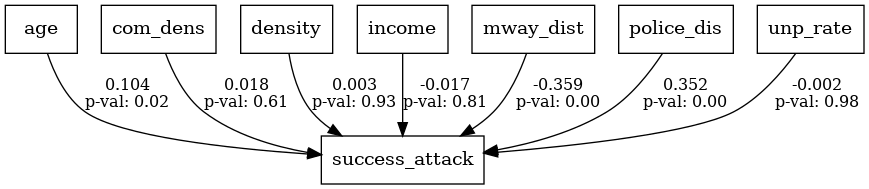
\includegraphics[width=\linewidth]{success.png}
		\caption{SEM Model}
		\label{fig:Model}
	\end{figure}
	
	In Figure \ref{fig:Model}, directional relationship from the predictor variables to the outcome variables is shown. 
	The tilde symbol \textasciitilde,  indicates a directional relationship from the predictor variables to the outcome variable. Essentially, it specifies that success\_attack is regressed on the other variables listed on the right-hand side of the formula.
	
\begin{enumerate}
	\item Name of objective: (ULS) unweighted least square 
	\item  Optimization method: SLSQP
	\item  Objective value: 0.000
	\item  Number of iterations: 50
\end{enumerate}	
\textbf{Equation used}
\begin{subequations}
	\begin{align}
		\begin{split}
			\text{success\_attack} \sim &\, com\_dens + \\
			&\, age + income + \\
			&\, unp\_rate + density + \\
			&\, police\_dis + mway\_dist
		\end{split}
	\end{align}
\end{subequations}

\begin{table}[htbp]
	\centering
	\caption{Parameter Estimates}
	\label{tab:parameter_estimates}
	\begin{tabular}{
			l
			S[table-format=1.6] % Adjust the number of digits before and after the decimal point as needed
			S[table-format=1.6]
			S[table-format=2.6]
		}
		\toprule
		 Variable & {Estimate} & {Std. Error} & {z-value} \\
		\midrule
		success\_attack $\longrightarrow$ com\_dens & 0.000337 & 0.000656 & 0.513490 \\
		success\_attack $\longrightarrow$ age & 0.003073 & 0.001354 & 2.270089 \\
		success\_attack $\longrightarrow$ income & -0.000414 & 0.001723 & -0.240056 \\
		success\_attack $\longrightarrow$ unp\_rate & -0.000102 & 0.004123 & -0.024623 \\
		success\_attack $\longrightarrow$ density & 0.000084 & 0.000998 & 0.083945 \\
		success\_attack $\longrightarrow$ police\_dis & 0.000324 & 0.000032 & 10.049766 \\
		success\_attack $\longrightarrow$ mway\_dist & -0.000111 & 0.000014 & -8.217081 \\
		\bottomrule
	\end{tabular}
\end{table}

\begin{enumerate}
	\item DoF: 28
	\item chi2: 0.0000004704235
	\item chi p-value: 1
	\item CFI: 1
	\item GFI: 1
	\item RMSEA: 0
\end{enumerate}







\section{Model}	
\begin{figure}[H]
	\centering
	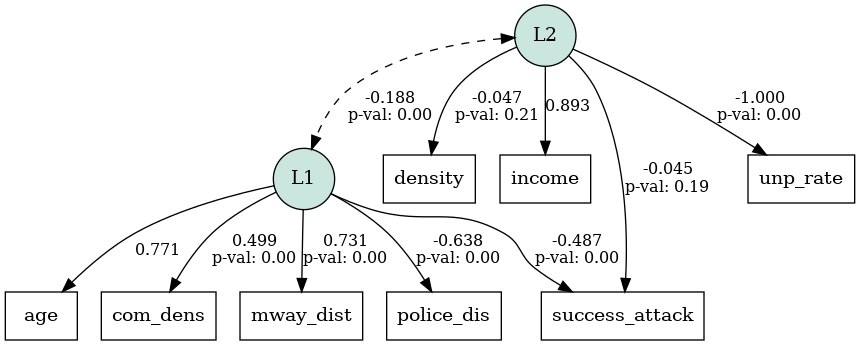
\includegraphics[width=\linewidth]{semoutput.png}
	\caption{SEM Model}
	\label{seml}
\end{figure}


In figure \ref{seml}, we can conclude that commercial density, age, police distance, motorway distance are emerging as significant factors for predicting success of attack.



\begin{enumerate}
 \item objective: (DWLS) Diagonally weighted least square 
 \item Optimization method: SLSQP
 \item Objective value: 0.187
 \item Number of iterations: 124
\end{enumerate}

\begin{subequations}
	\begin{align}
		\text{L1} &=\sim com\_dens + \nonumber \\
		&\quad age + income + \nonumber \\
		&\quad unp\_rate + density + \nonumber \\
		&\quad police\_dis + mway\_dist \\
		\text{L2} &=\sim income + unp\_rate + density \\
		\text{success\_attack} &\sim \text{L1} + \text{L2}
	\end{align}
\end{subequations}



\begin{table}[htbp]
	\centering
	\caption{Parameter Estimates}
	\label{tab:parameter_estimates}
	\begin{tabular}{
			l
			l
			l
			S[table-format=2.6] % Adjust the number of digits before and after the decimal point as needed
			S[table-format=1.6] % Adjust the number of digits before and after the decimal point as needed
			S[table-format=2.6] % Adjust the number of digits before and after the decimal point as needed
		}
		\toprule
		Variables & {Estimate} & {Std. Err} & {z-value} \\
		\midrule
		age $\longrightarrow$ L1 & 1.000000 & null & null \\
		police\_dis $\longrightarrow$ L1 & -22.312517 & 1.467501 & -15.204427 \\
		mway\_dist $\longrightarrow$ L1 & 86.185086 & 5.060644 & 17.030458 \\
		com\_dens $\longrightarrow$ L1 & 0.950915 & 0.074655 & 12.737455 \\
		income $\longrightarrow$ L2 & 1.000000 & null & null \\
		unp\_rate $\longrightarrow$ L2 & -0.473068 & 0.065219 & -7.253544 \\
		density $\longrightarrow$ L2 & -0.029171 & 0.033489 & -0.871065 \\
		success\_attack $\longrightarrow$ L1 & -0.015681 & 0.001504 & -10.426593 \\
		success\_attack $\longrightarrow$ L2 & -0.001003 & 0.000951 & -1.054167 \\
		\bottomrule
	\end{tabular}
\end{table}

\begin{enumerate}
	\item DoF: 18
	\item chi2: 135.306313
	\item chi p-value: 0
	\item CFI: 0.935434
	\item GFI: 0.926657
	\item RMSEA: 0.095007
\end{enumerate}

\subsection{Relation explanation}

\textbf{L1 and L2:} These are latent variables in the model. Latent variables are not directly observed but are inferred from observed variables (we have divided the observed variables in two sets) . In this context, L1 and L2 represent underlying  factors that are influencing the observed variables. The value of -0.188 represents the estimated correlation coefficient between the two latent variables. In this case, a negative correlation coefficient suggests that as one latent variable increases, the other tends to decrease, and vice versa.\\
The regression path from L2 to "success attack" is not statistically significant.\\
The regression path from L1 to "success attack" is statistically significant, indicating a significant negative relationship between L1 and "success attack".\\

The covariance between L1 and L2 indicates the degree of correlation between the two latent variables beyond their individual relationships with observed variables. A negative covariance suggests an inverse relationship between L1 and L2, indicating that higher values of one variable are associated with lower values of the other. This suggests that factors influencing L1 may have an impact on L2, and vice versa, beyond their direct relationships with observed variables.\\

Based on the information obtained, it seems plausible to infer that L2 may not have a direct effect on "success attack" but might influence it indirectly through its influence on L1. This interpretation aligns with the idea of mediation in SEM, where one variable (L1) mediates the relationship between another variable (L2) and an outcome (success attack).\\


\textbf{Relation between Factors}

Commercial density (com\_dens), age, police distance (police\_dis), and motorway distance (mway\_dist) all show statistically significant relationships with the latent variable L1, which represents a construct related to community well-being. These relationships suggest that certain demographic and geographic characteristics, such as higher commercial density, older populations, greater police presence, and increased distance from major highways, may contribute to lower rates of successful attacks.\\
Additionally, the observed variables income, unemployment rate (unp\_rate), and population density (density) show significant relationships with the latent variable L2\\


The significant relationships observed in the SEM model underscore the complex interplay between geographic, demographic and economic factors in influencing success of attack. 




\end{document}